\documentclass[main.tex]{subfiles}
\graphicspath{{./img}}

\begin{document}
    
\section{Proposed system}\label{sec-system}

This section is dedicated to designing the system that will be used to implement ITS in the
vehicle simulator software. A framework dedicated for generic MAS-based ITS system
implementation will be designed, utilizing the principles and paradigms gathered in the
preceding sections (\ref{its}, \ref{mas}). Firstly, the \emph{micro-architecture} will be
defined, i.e. the specification of the system's actors (agents) - their features,
characteristics, state variables and their goals, as well as interfaces to the environment.
This will form the elementary foundation that will be used to build an actual system. As a
follow up, agent interaction interface will be defined. This will for example include
knowledge sharing, conflict resolution and overall communication interface proposal, including
shared vocabulary and communication layers definition. The interaction interface will,
subsequently, lead to the \emph{macro-architecture} proposal. The structure of the system and
will be defined. These steps should lead to a full system specification that will serve as a
framework to implement agent-based ITSs in an interactive vehicle simulator.

\subsection{Agent/micro architecture overview}

As per the previous section(s), where the individual MAS architectures have been reviewed
(section \ref{mas}), it was decided to utilize  the hybrid \emph{\textsubscript{3}T
architecture\footnote{To remind the reader of the architecture's general structure, its
schematic is shown below (fig. \ref{3-arch2}).}} (section \ref{hybrid-arch}), which will offer
sufficient flexibility.  Such modeling flexibility is needed primarily because there won't be a
single, concrete system to model, but rather a generic system that will facilitate arbitrary
agent-based ITS implementation. As such, it makes sense to choose a hybrid architecture, which
will ensure there will be optimal balance between robust, reactive behaviour without giving up
capabilities to model complex behaviour.

Note that the architecture will be formally assume that the its implementation will be realized 
in an Object-Oriented Programming (OOP) paradigm. There are multiple reasons for that. Firstly, 
The nature of agent based systems, having their internal logic and interacting with the surroundings 
through pre-defined interface, corresponds to a large degree to the concepts of OOP, especially
the encapsulation mechanism.

The individual layers/components will be outlined in the following section, in a bottom-up
fashion.

\begin{figure}[htbp]
    \centering
    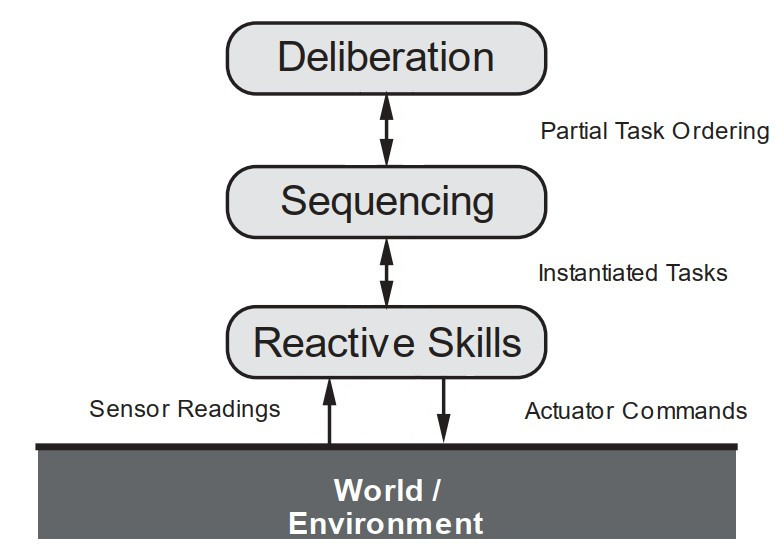
\includegraphics[width=.8\textwidth]{3t-arch.jpg}
    \caption{An architecture model of a \textsubscript{3}T hybrid architecture \cite{Bonasso1995}}
    \label{3-arch2}
\end{figure}

% The elementary characteristics that were defined according to \cite{ParasumannaGokulan2010}
% must shall also be taken into account: 

% \begin{itemize}
%     \item Situatedness
%     \item Autonomy 
%     \item Inferential capability 
%     \item Social behaviour 
% \end{itemize}

\subsubsection{The architecture layers}

In this section, the individual layers of the architecture will be defined. The layers' definition will 
adhere to the characteristics of the \textsubscript{3}T architecture. For each layer, it's purpose and 
relation to other layers will be described, together with technical implementation guidelines, such as 
configuration etc.

\textbf{Reactive skills layer \\\& Physical modules}

This layer encapsulates all the \emph{skills} the agent is able to do. These are the 
most primitive types of its behaviour\footnote{The original author of the architecture refers to them 
as Reactive Action Packages (RAPs) \cite{Firby1987}.}. For example, a skill might be to slow
down or to follow a vehicle in case of vehicle-based agent. Skills are usually activated one at a time, 
activated by the superior layers. This creates a level of abstraction, comparable to the principle found 
in Object Oriented Programming, where the superior unit (sequencer in this case) does not care how the 
given instruction will be executed. The sequencer only cares about the use-case and output of available
skills. 

In practice, each skill will be an individual script that will be synchronously, sequentially run. Inside 
the script, it will be possible to interact with the agent's interface, mainly its sensors or communication 
modules. The sensor and communication modules may provide an additional level of abstraction,
with exposed interface which will be defined by the architecture but configurable by the user.
This will mostly involve defining parameters of physical characteristics of the module, such 
as signal range, or error rate. Speaking of error rate, a skill will be also able to return a 
failure state to enable fail-safe behaviour. 

This essentially means that the skills will interact with another layer, which we could call the
\emph{Physical module layer}. This will be an elementary unit, which must be bound to a specific agent type. 
Therefore, the assigned modules will determine which skills the agent will be able to perform.  

\textbf{Sequencing layer}

The sequencing layer is responsible for \emph{queue management} and \emph{execution} of the individual skills. It is the 
intermediate layer between the reactive skill layer and deliberative planning layer. 

Apart from the trivial FIFO skills queuing, the sequencer will manage concurrent queues with different 
priorities, as the agent has to conform to a dynamic environment. Because indirect communication (i.e. 
broadcasting) will be featured in the proposed system, asynchronous skill sequencing will also be 
implemented using \emph{callbacks}. Usage of this feature can be simply argued by the fact that in traffic, 
the state of environment is changing rapidly, thus relying on sensory feedback would often not be enough 
to avoid faulty behaviour. Furthermore, there is a vast number of ITS solutions that utilize the 
broadcaster-subscriber principle, such as CACC systems and C-ITS systems in general.

\textbf{Deliberation layer}

The deliberation layer (planner) synthesizes high-level goals into a partially ordered \emph{plan}, listing tasks that 
the agent has to perform, in order to achieve the specified goal. For example, A vehicle's goal is to get from 
its initial position to its destination. The deliberation initializes a plant which sequences skills that 
should ensure the vehicle gets to the destination point. The deliberation layer is aware of the traffic network 
(i.e. the environment), but hasn't got \emph{complete knowledge} about it. In other words, the agent knows which turns
to take on the network to get to the destination, but isn't aware of every vehicle, pedestrian or other "obstacle" that 
could get in its way. That's why, when there is, for example, a slow vehicle that can be overtaken, the deliberation layer 
\emph{replans} the tasks in order to resolve the situation. 

In practice, the deliberation component in this proposed framework will contain the most amount
of pre-defined logic.  The deliberation layer will contain solutions to actual problems,
creating \emph{workflows} created from individual steps (skills).

The most trivial option will be to create \emph{static} workflows, which will work under the
assumption that workflow will not get interrupted or reach a fail state at any point, i.e. is
expected to finish. The second option will be to create \emph{dynamic} workflows, which will enable
re-planning according to changing environment conditions.  Re-planning will occur when it's
triggered by one of the \emph{exit state} of agent's skills. The triggers will happen under the
following conditions: skill returning a \emph{failure state}, callback triggered by a broadcast
subscription or result of inter-agent negotiation (discussed later). This will cause the
planner to re-plan by adding appropriate steps to the executing workflow to optimally adapt to
the situation. Therefore, the framework will offer to define conditions under which additional
steps will get added to ideally achieve a \emph{fail-safe behaviour}. For better logical
organization, the added steps (which are identified to most often execute in a certain
sequence) could be grouped into \emph{subtasks}.

To further improve the resilience of the
system, the executing workflow can be configured to reach a \emph{workflow failure state},
which will trigger a pre-determined fail-safe workflow, that is composed of entirely different
steps, essentially throwing away the previous, failed workflow.  This will be useful when the
planner will run out of options to adapt to the situation, settling for a goal that would
destabilize the system as least as possible. For example, autonomous vehicles performing a
\emph{minimum risk maneuvre} to come to a standstill on the road side when the expected driver
input is not received \cite{WorkingAutonomous2022}.

A more detailed view on the individual components of the architecture is on the image (\ref{3t-arch-detailed}) below.

\begin{figure}[htbp]
    \centering
    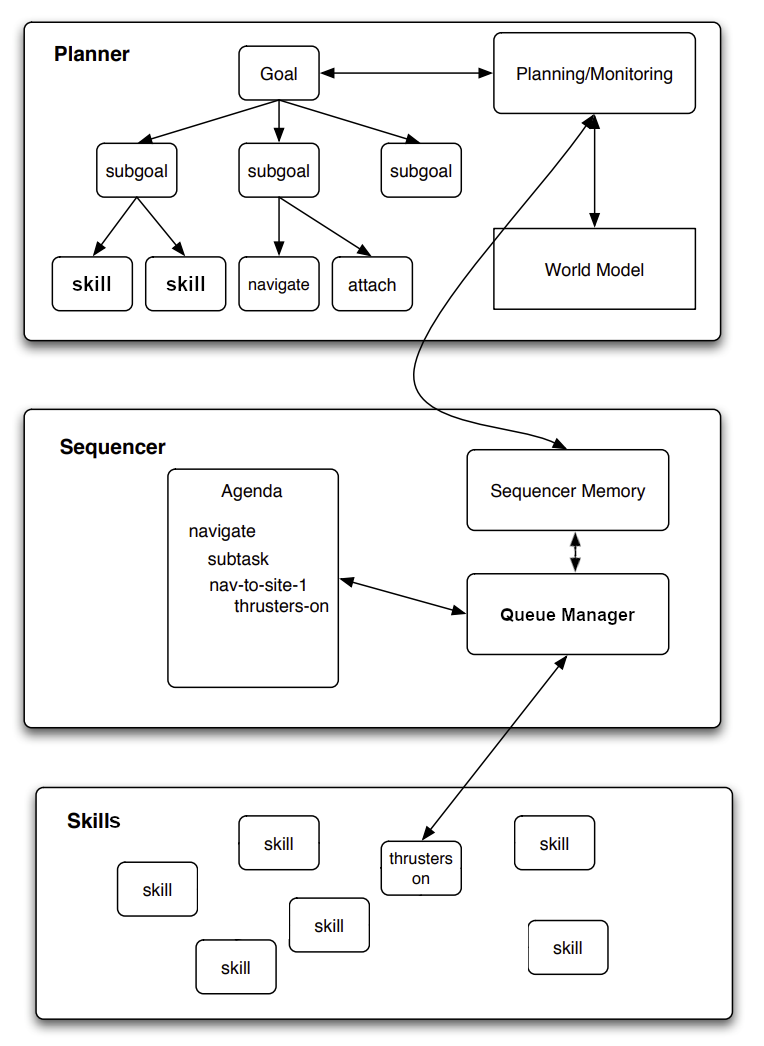
\includegraphics[width=.8\textwidth]{3T-arch-edited.png}
    \caption{An overview of the proposed 3T architecture \cite{Binder2022} (\emph{edited})}
    \label{3t-arch-detailed}
\end{figure}
\pagebreak
%%%%%% I'd move this further down to the full implementation phase
% Firstly, the matter of how much logic has to be pre-defined in the framework and how much will be left to the implementation 
% itself needs to be discussed thoroughly in this case, as there is a non-trivial task. The



\subsection{Macro architecture}

\subsubsection{Communication protocol}

As has been discussed in the previous sections, communication plays an important part in 
MAS, mainly because it vastly extends capabilities of interaction between agents and thus 
the ability to model more complex behaviour. In section (\ref{sec-acl}), the ACL communication 
standard for MAS has been introduced and requirements for the protocol implementation have 
been presented. To be able to 
utilize the communication, requirements for messaging utility and high-level implementation 
details will be presented. 

\subsubsection{Broadcasting}

The first type of communicating that will be implemented is message broadcasting. This is 
argued by the fact that ITS uses information broadcasting in a lot of cases.
Generally, ITS services have common communication requirements \cite{Santa2013}:

\begin{itemize}
    \item \textbf{Periodic status exchange} - ITS services often need to know about 
    status of other actors, such as terminals or vehicles. These periodic updates 
    often include basic status messages such as location, ID, speed, etc.
    \item \textbf{Asynchronous notifications} - Messages that are used to inform 
    about specific event, usually related to a specific service and functionality.
\end{itemize}

%  Especially the C-ITS platform, which uses two types of (middleware) messages,
% specified by the European Telecommunication Standards Institute (ETSI):

% \begin{itemize}
%     \item \textbf{Cooperative Awareness Message (CAM)} which are "heartbeat" periodically 
%     broadcasted messages
%     \item \textbf{Decentralized Environmental Notification Message (DENM)} which are event-
%     triggered messages broadcasted to alert road users.
% \end{itemize}

The framework should therefore support message broadcasting for both synchronous and 
asynchronous events, which should ensure that all potential use-cases are covered. 

As has been mentioned above, the ability to broadcast and subscribe to said broadcast should be
handled by a separate "physical module" that will be active throughout execution of individual
skills, i.e.  its lifetime should not depend on other skills lifetime. An exception to this
would be the skills whose purpose is to \emph{register} and \emph{un-register} those
communication modules.  The broadcast and subscription will work like most such communication
systems, where each agent chooses a stream to connect to and publish/consume messages from
queue (with pre-defined semantics i.e. CAM, DENM). The ability to act upon a received message
will be also implemented, by making a callback that makes the skill end and return. 

\subsubsection{Negotiation \& Agreement}
% still quite too theoretical, not related to actual implementation. not sure if it should be here
Negotiation between agents is important especially when wo agents run into each other, 
followed by the currently executing skills of the agents getting interrupted. In other words, 
The best course of action of one agent is not necessarily best to the other. This is more than
likely to happen in environments where multiple agents share the same resource and their state
is defined on the same domain, which is often the case. As such, the theory of games is formally 
used to model these interactions \cite{Binder2022}. 

This is quite different from the principles of agent cooperation. In cooperation negotiations, 
the worst-case scenario improvement as opposed to working individually is net-zero. \cite{Binder2022}
defines four speech acts in agent negotiation, as seen on fig. (\ref{fig-speech-acts}). This is 
inherently contrary to the statement made in chapter (\ref{mas-interaction}), where it was suggested 
that agent cooperation should be emphasized. However, as agents are formally modelled as self-interested, 
it cannot be guaranteed that they won't encounter conflicts between each other. Therefore, modelling 
cooperation before figuring conflict resolution would inherently result in a more fragile system 
more prone to malfunction. 

\begin{figure}[htbp]
    \centering
    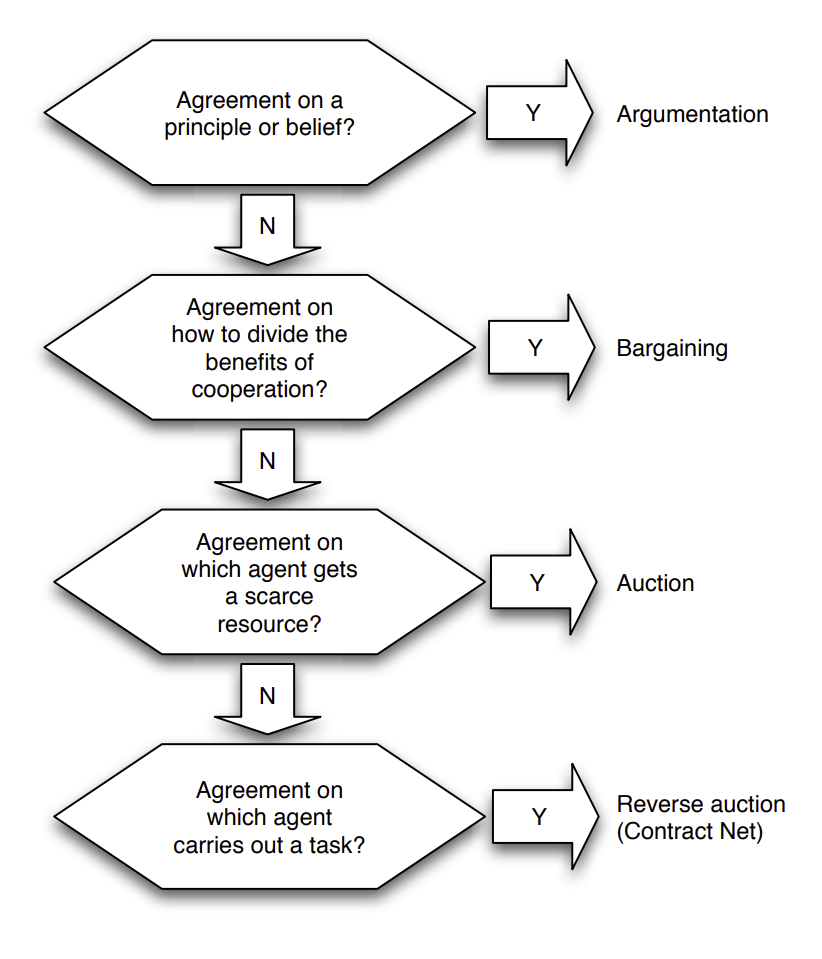
\includegraphics[width=.8\textwidth]{speech-acts.png}
    \caption{Types of agent negotiation \cite{Binder2022}}
    \label{fig-speech-acts}
\end{figure}

\subsubsection{Conflict detection}

As has been argued above, because of scope limitation of this thesis, 
conflict resolution as a system functionality should precede cooperation. The cooperation 
abilities of agents can be added later by extending the framework.
This decision will theoretically lead to better system stability, before offering extended
behaviour possibilities. 

The first step is to have a way for agent to determine a conflict has happened. Agents wouldn't be 
able to resolve conflicts if they didn't know it has occurred. To comply with the \textsubscript{3}T
architecture topology defined above, this should be handled on the reactive skills layer. 
Consequentially, detected conflict will be handled through a aforementioned module that will be bound 
to an executing skill. If an agent is expected to run into a conflict with another agent (of the same 
type), if will have to be "equipped" with a dedicated module that will behave as a sensor detecting conflict 
with the implementation left to specific use-case. In other words, the logic for conflict detection will be 
left to define together will specific agent and its properties, and other modules.

This will make the conflict detection process very flexible, as agent will have the "luxury" to combine
his sensory feedback with communication modules to detect conflict with another agent. This will also 
solve the potential issue with only one agent acknowledging there is a conflict between it and 
other agent(s). Namely when one agent detects a conflict through one of its modules, it can inform 
other agents about the conflict as a consequence and all agents will be aware of the situation. 

%add an image? 

\subsubsection{Conflict resolution}

Now that the conflict detection process was defined, in that case, it will be possible to build
on it to define how conflicts will be resolved. Considering the findings in chapter \ref{sec-conflicts},
the best tool to resolve conflicts is to define hierarchy in the agent. That is, assigning each agent a 
hierarchical level that determines his bidding power. As the figure (\ref{fig-speech-acts}) depicts, 
when . In relation to the figure (\ref{fig-speech-acts}), conflict is essentially a a competition about a 
resource. The said resource can have many forms apart from the more obvious free space (fig. (\ref{agentReplanning})),
more generally, it can also be defined as a right to decide first what action to take, on the expense of the other agent(s) in 
the conflict. In order to avoid more complex mathematical reasoning models \cite{Binder2022}, we can determine the bidding 
power by one or more agent-bound resource types that each have a value assigned. This value can be either predefined 
(e.g. hierarchical level) or change dynamically based on agent state and the surrounding environment (e.g. relative 
position of the agent). 

\textbf{Example}

To illustrate how the system would work in practice a sample scenario is presented below on
figure (\ref{agentReplanning}), where the agents are drivers/vehicles. The scenario demonstrates 
how agents achieve their goals using the three layers, as well as conflict detection and resolution.

There are two vehicle agents (\texttt{A}, \texttt{B}) in the scenario, which both have three skills defined:
\texttt{drive}, \texttt{avoid:object} and \texttt{wait} and \texttt{negotiate}. Both vehicle
agents have a goal not to crash and keep a certain speed. To ensure a fail-safe behaviour, a
dynamic workflow is used, defined as a mapping
(\texttt{failed\_skill}$\rightarrow$\texttt{safe\_skill}): 

\begin{itemize}
    \itemspacing{.5}
    \item \texttt{drive} $\rightarrow$ \texttt{avoid:object}
    \item \texttt{avoid:object} $\rightarrow$ \texttt{wait}
    \item \texttt{wait} $\rightarrow$ \texttt{fail\_goal} (after a timeout for example)
\end{itemize}

The mapping of the \texttt{negotiate} skill is \texttt{drive} or \texttt{wait} based on 
a negotiation result for each involved agent.

\begin{enumerate}
    \item Both agents do not detect any obstacles in their surroundings, so the planner
    initializes a plan with only the \texttt{drive} skill sequenced, which gets executed. 

    \item Agent (\texttt{A}) spots an obstacle in his way (an oil spill). This makes the
    \texttt{drive} skill fail and (\texttt{A})'s planner has to re-plan to reach its goal (not
    crash). The failed skill's fail-safe skills are retrieved (\texttt{avoid:object})
    and added to the new plan. The new plan is initialized with the two
    following skills sequenced: \texttt{avoid:oil\_spill} $\rightarrow$ \texttt{drive}.
    
    \item However, this plan also fail, as agent (\texttt{B}) detects a path conflict, consequentially 
    informing agent (\texttt{A}) about it. They now have to negotiate to reach an agreement and
    resolve the conflict using auction-like bidding. The agent (\texttt{B}) wins the bid, due
    to being in a right lane and so agent (\texttt{A}) is forced to give way. The planner
    creates a new plan: \texttt{wait} $\rightarrow$ \texttt{avoid:oil\_spill} $\rightarrow$
    \texttt{drive}.
    
    \item The individual skills finish successfully and the agents' goal is fulfilled.
\end{enumerate}

\begin{figure}[htbp]
    \centering
    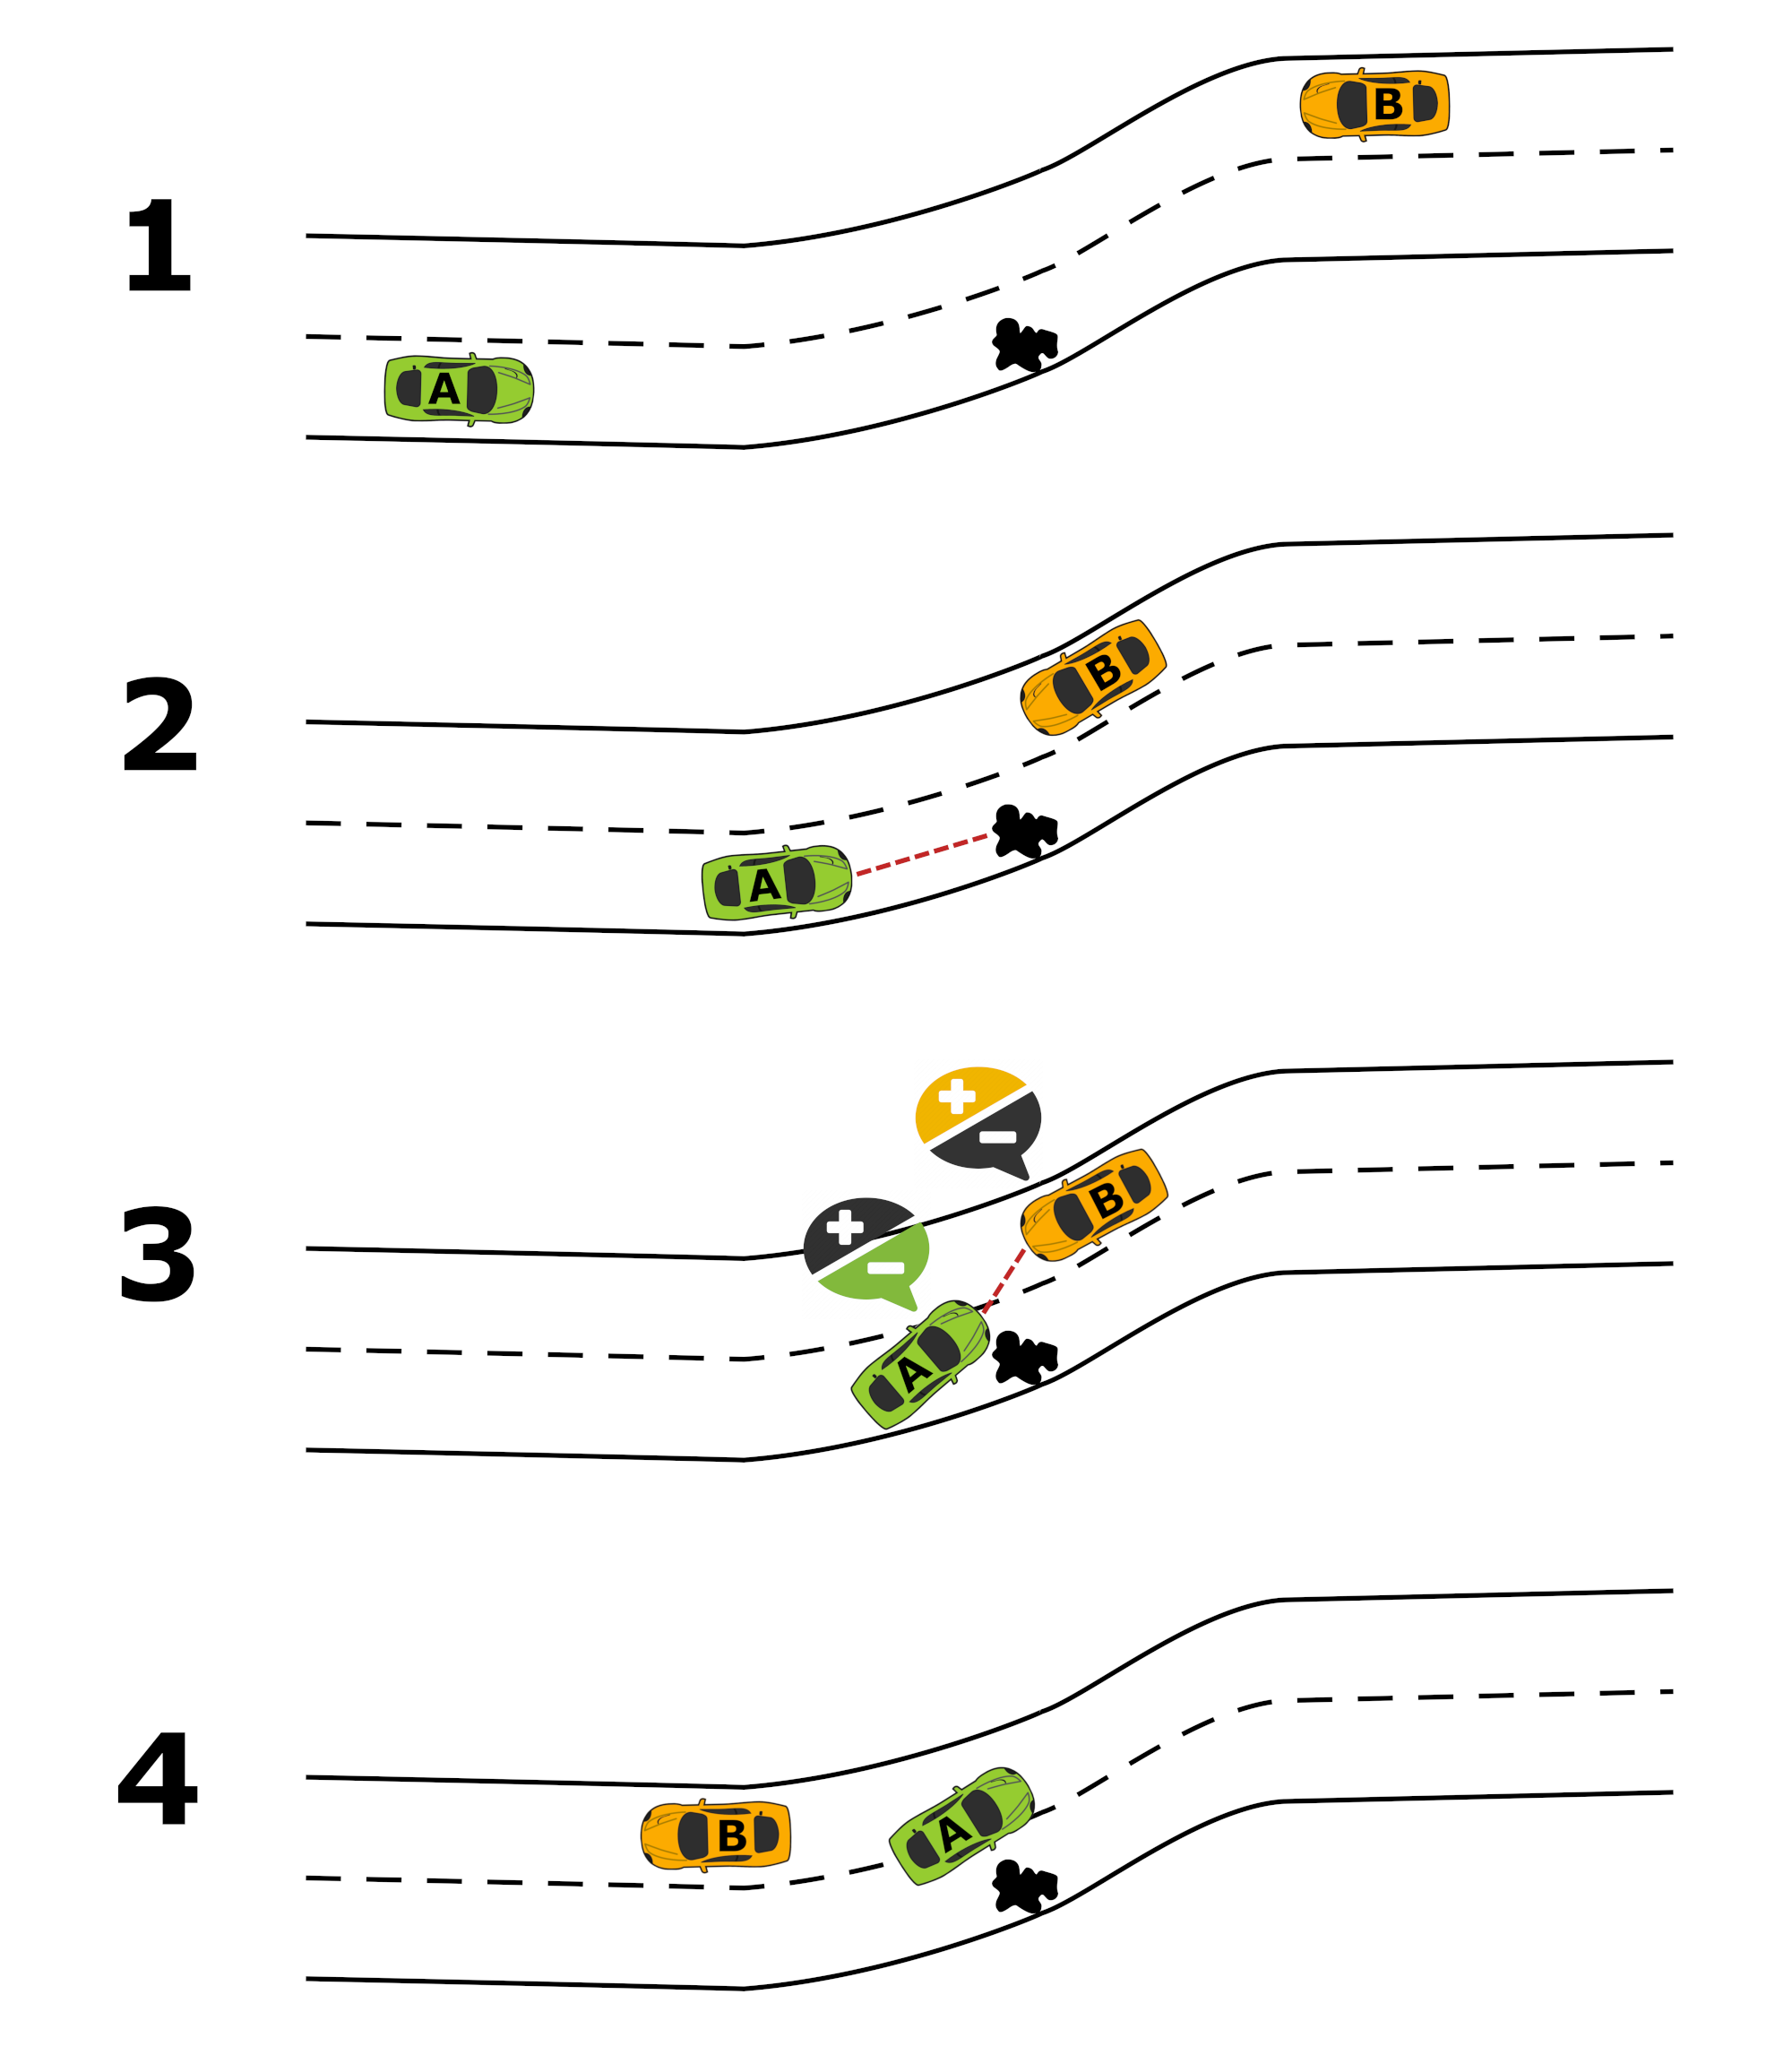
\includegraphics[width=.8\textwidth]{AgentPlanning.png}
    \caption{An example behaviour of vehicle-based agents using the proposed architecture}
    \label{agentReplanning}
\end{figure}

\subsection{System requirements}

To sum up the topic discussed in previous chapters, requirements for framework implementation will be 
concluded. This will ensure that when integrating this ITS framework into existing system (i.e. IVS 
software), the requirements will be organized and kept as a reference, helping achieve the desired 
functionality. Especially when later choosing a library/framework to help build the framework. 

\begin{table}[htbp]
    \caption{Proposed system requirements}
    \centering\begin{tabular}{>{\footnotesize}p{.9\textwidth}}
        \toprule
\textbf{Requirement 1}: The framework should be a multi-agent based system, supporting more actors 
that are able to act independently, having their own logic and able to make decisions based on their 
own perception of the environment.
\\ \midrule
\textbf{Requirement 2}: The framework should support the \textsubscript{3}T architecture. 
This primarily means implementation of the three layers of logic that offer complex behaviour 
modelling.
\\ \midrule
\textbf{Requirement 3}: The framework's architecture should be modular enough to support broad 
spectrum of ITS implementation.
\\ \midrule
\textbf{Requirement 4}: The actual implementation of a particular actor's abilities should be done using 
elementary skill modules.
\\ \midrule
\textbf{Requirement 5}: An agent should be able to interact with the environment using physical modules 
that are bound to individual skills. The physical sensor modules should have a given interface to provide 
expected output and/or input. 
\\ \midrule
\textbf{Requirement 6}: Agent should be able to communicate with others through a dedicated communication 
interface, with pre-defined semantics. The communication should also adhere to the ACL-compliance requirements 
mentioned in section \ref{sec-acl}. 
\\ \midrule
\textbf{Requirement 7}: The supported communication modes will be both direct (messaging specific agents) and indirect  
(broadcast \& subscription). 
\\ \midrule
\textbf{Requirement 8}: Agent should be able to act upon received information from physical
modules, i.e. sensors and communication interface. That means, being able to process received
information on skill-level, and signaling to the deliberation layer appropriately. 
\\ \midrule
\textbf{Requirement 8}: Execution of the elementary skills should be managed by the sequencing layer. 
The sequencing layer should provide interface to facilitate such management. 
\\ \midrule
\textbf{Requirement 9}: Each agent should have its role determined by defining its workflows. The workflows 
are series of steps that should finish as soon as the agent reaches its main goal. 
\\ \midrule
\textbf{Requirement 10}: It should be possible for an agent to adapt to the environment by dynamic re-planning.
this will be achieved by offering conditional sub-tasks that will be managed by the conditional logical reasoning 
system in the deliberation layer.
\\ \midrule
\textbf{Requirement 11}: Execution of these conditional sub-tasks should be based on exit states of individual skills.
\\ \midrule
\textbf{Requirement 12}: The deliberation layer should be able to process all skills' exit codes that were defined. 
\\ \midrule
\textbf{Requirement 13}: It should be possible to implement a fail-safe behaviour, which gets activated in case 
the specified goal cannot be reached by the agent. In such case, a specific fail-safe workflow is defined. 
\\ \midrule
\textbf{Requirement 14}: Where applicable, agents should be able to detect conflicting intentions with other agents
while executing their tasks. The conflict detection will be implemented as a module on the reactive layer.
\\ \midrule
\textbf{Requirement 15}: On conflict-detecting agents, they must come with a communication module, to be able to 
notify other about the conflict or receive such notification. 
\\ \midrule
\textbf{Requirement 16}: Conflict-detecting agents should be either able to resolve the conflict or trigger fail-safe 
state. 
\\ \midrule
\textbf{Requirement 17}: Conflict resolution should be done by bidding a pre-defined resource(s). Hierarchy level can 
also count as a resource.
\\ \bottomrule
    \end{tabular}
    \label{sys-requirements}
\end{table}

\subsection{Conclusion}

In the preceding sections, the multi-agent system framework was proposed. This framework will be used to implement various 
suitable ITSs into an interactive vehicle simulator. The system was described both on micro and macro level. The micro level 
mainly addressed specification of inner architecture of individual agents, how they will achieve their goals using their 
own intelligence. For building independent agents that need to be flexible in terms of their capabilities, the \textsubscript{3}T
architecture was chosen and the individual layers of the architecture were specified in detail, specifying their responsibilities
and capabilities. 

Afterwards, the macro architecture was specified, addressing mainly the ways of how agents will interact with each other. 
Firstly, the communication interface was defined, including how agents will be able to use it on micro-architecture level.
Building upon that, the ways of how conflicts between agents are handled was proposed, utilizing communication to resolve 
conflicts through resource bidding. 

With the micro- and macro-architecture being specified, the final requirements for the system implementation were proposed, 
which aim to help ensure that the software framework will be able to facilitate ITS implementation into IVS software in an 
organized way, with a high system resilience.

\section{System implementation}

With the finished system specification, it should be discussed which tools should be used to build the software framework. 
First off, it is important to analyze the IVS simulation system/software (i.e. the super-system) that
the proposed framework will be incorporated into. An effort should be made to maximize the super-system acceptance of 
this system by choosing an optimal tool-set for its implementation. This, for the most part,
refers to an optimal choice a programming language and a subsequent agent-based modelling
library to use (if there will be any), also due to this being one of the primary tasks of this thesis. 
Therefore, the next section will be devoted to introduction to the IVS software.

\subsection{Simulator software}

The particular simulator software that is being used at the university's faculty is being
developed using the \emph{Unity} game engine, developed by Unity Technologies. The game engine
was first released in 2005 and has been used to develop numerous simulators as well as other
video games ever since \cite{UnityTechnologies2022}.  Unity has also been used as a tool in
physical product modelling, AI \& machine learning and digital twins, used in many industries
\cite{UnityTechnologies2022a}.  The main strengths of Unity are multi-platform development
support, virtual reality development support, good community support (including its own asset
store) and good documentation. The game engine has got its own development environment, which 
can be seen on figure (\ref{unity}) below.

The game engine's runtime is written in the C++ programming language, but the scripting API 
that it offers is in the C\# language. Consequently, the libraries that will be used to develop 
the system should ideally also be .NET based to achieve maximum customization and interoperability.
Potentially, the Unity's Asset store could offer MAS packages, directly utilizing Unity's API.

\begin{figure}[htbp]
    \centering
    
    \caption{The Unity development platform UI}
    \label{unity}
\end{figure}

\end{document}
